\documentclass[11pt,conference,onecolumn]{article} %This uses the IEEE template

%Set up for inputing Figures
\usepackage[margin=1in]{geometry}
\usepackage[pdftex]{graphicx}
\usepackage{wrapfig}
\usepackage[utf8]{inputenc}
\usepackage{mathptmx}
%Include math packages
\usepackage{algorithm}
\usepackage[noend]{algpseudocode}
\usepackage{amssymb}
\usepackage{amsmath}
\usepackage{latexsym}
%Added Recommended packages
\usepackage{csquotes}
\usepackage[backend=biber]{biblatex}
\usepackage{hyperref}
\usepackage[noabbrev]{cleveref}
\usepackage{lscape}
%Include packages for line spacing
\usepackage{setspace}
\usepackage{parskip}
\usepackage{indentfirst}
\usepackage{verbatim}
\usepackage{adjustbox}
\usepackage{listings}
\usepackage{subfigure}
\usepackage[T1]{fontenc}
\usepackage[scaled]{beramono}
\usepackage[tableposition=top]{caption}
\usepackage{sectsty}

\captionsetup[figure]{labelfont=bf,labelsep=period}
\captionsetup[table]{labelfont=bf, labelsep=newline, font=sc}
\subsectionfont{\normalfont\large\bf\underline}

\newcommand\Small{\fontsize{9}{9.2}\selectfont}
\newcommand*\LSTfont{\Small\ttfamily\SetTracking{encoding=*}{-60}\lsstyle}
\def\BState{\State\hskip-\ALG@thistlm}
\addbibresource{/home/ivan/Documents/Latex_Stuff/BibDB/AllEntries.bib}
%dont think I need to use the graphics path yet
\graphicspath{{/home/ivan/src/Internship_GTRI/Documentation/Images/}
{/home/ivan/src/Internship_GTRI/Documentation/Images/screenshot/}} %Change this to your path!!!

\DeclareGraphicsExtensions{.pdf,.jpeg,.jpg,.png} %Make sure your figure extension is included in this list

%simple command to add a figure
%\myfigure{address}{caption}{width}{label}
\newcommand{\myfigure}[4]{
  \begin{figure}[h!]
      \centering
      \includegraphics[width=#3\textwidth]{#1}
      \caption{#2}
\label{#4}
    \end{figure}
}

%simple command to add a figure wrapped in text
%\myfigure{image/address}{R_L_PLACEMENT}{width_in_text_width}{caption}{label}
\newcommand{\mywrapfigure}[5]{
  \begin{wrapfigure}{#2}{#3\textwidth}
    \centering
    \includegraphics[width=#3\textwidth]{#1}
    \caption{#4}
\label{#5}
  \end{wrapfigure}
}

\newcommand*{\figuretitle}[1]{%
    {\centering%   <--------  will only affect the title because of the grouping (by the
    \textbf{#1}%              braces before \centering and behind \medskip). If you remove
    \par\medskip}%            these braces the whole body of a {figure} env will be centered.
}

%Set up spacing
\linespread{1.3} %This creates 1.5 spacing
\setlength{\parindent}{12pt} %Sets the length of the indent at the beginning of each paragraph.

%Start the document
\begin{document}

\title{\vspace*{30mm}
An Incremental Approach to DE2Bot Robot Navigation}

\author{
Millun Atluri,\\
Mitchell Reid Donley,\\
Nicholas Fahrenkrog,\\
Ivan Dario Jimenez
\vspace*{30mm}\\
ECE2031 Digital Design Lab,\\
Section L03\\
\vspace*{30mm}\\
Georgia Institute of Technology\\
School of Electrical and Computer Engineering\\
Submitted: \today
}

\clearpage\maketitle

% Executive Summary
% This section should be one paragraph (not multiple), approximately ½ page in length.  The Executive Summary summarizes the entire document – it clearly and explicitly states what type of document this is (design report, comparison report, feasibility study, technical review, etc.) and explains what is being designed, reviewed, proposed, or compared.  A reader should know exactly what you plan to do and how you plan to do it, and the significance of the work after reading your ES.  You’re not writing a mystery novel.  Tell the reader up front, in one paragraph, what this document is about and why it is worth their time to read.
\section*{Executive Summary}
This proposal will guide the reader through \emph{Firmly Grasp It}'s approach to complex point-to-point navigation in the DE2Bot. This task entails making the DE2Bot visit twelve arbitrary points given in a randomly ordered list. This list will be written by an operator to an xml file which a program will use to write the coordinates to the assembly file that is compiled and downloaded to the DE2Bot. For simplicity, this task will be divided into two parallel sub-problems: optimal path planning given the sequence of points and point-to-point travel. The initial solution for path planning will have the robot going to the points in the original list's order. A second solution will be a pre-computation program that takes the list of points and orders them using a greedy algorithm. If we determine that the point ordering is a critical inefficiency, the team will find a optimal path using a parallelized brute force solution. For the point-to-point navigation, an initial solution will make the robot turn until it is facing the target and then move forward until it reaches it. Finally, the team will attempt to implement a sophisticated algorithm that approximates the movements of the robot using circles to minimize the travel time. Since the initial approaches are simple to implement while still yielding a solution, the team will always be able to revert to a previous version in case there are unforeseen problems during the implementation of more advanced features.


\clearpage
% Descriptive Title (same as cover page)

\begin{center}
  
   \textbf{\LARGE An Incremental Approach to DE2Bot Robot Navigation}
\end{center}

\section*{Introduction}
% The document starts here in the introduction.  It is completely acceptable to repeat some of what you wrote in the ES here in the introduction, because the introduction should not depend on having read the ES.  This is the first time the reader is hearing what type of document this is, what is being designed or proposed, and how the design was approached.  Begin with a general but brief introduction of the topic, and then move into a discussion of more specific areas of interest.  The Introduction should include explicit statements such as “This report examines…” or “This document proposes….”
This document proposes an incremental approach to developing complex point-to-point navigation for the DE2Bot. The team will be given a list of 12 Cartesian coordinate points $X \in [-4,4]$ and $Y \in [-5,5]$ where units are in feet. The robot will be placed at the starting coordinate $(0,0)$ with an orientation $\theta_{robot} = 0^{\circ}$.This problem can be subdivided into two parallel sub-problems: path planning and point-to-point navigation. Notice that these are coordinates calculated from the internal odometer calculation which means that the team can safely ignore any error accumulated between that and a real coordinate frame.\par
The team will write the coordinates to a file that will be read by a pre-processing program which will insert the coordinates into the assembly that is downloaded to the DE2Bot. This pre-processing step will be initially solved by writing the coordinates in the original order in which they are given. A second approach will use a greedy algorithm to order the coordinates. If the team determines the path is a critical point of inefficiency the team will attempt a parallelized brute force solution to find the  optimal path.\par
The point-to-point navigation will be initially solved by making the robot turn to face the target point and advance to cover the distance between the current point and the destination. Once this approach has been show to work, the team will implement an algorithm where the trajectories between points are taken to be smooth arcs. This final solution promises to be much more efficient since the robot will not have to stop moving between points to turn but will rather turn as it approaches the destination.\par


\section*{Technical Approach}

% Explain the process and steps you will take to solve the problem.  Organize this section using descriptive subheadings so that the reader can easily find the components of the design.  Use figures, bullets, enumerated lists, or tables to organize information (you don’t always have to write a paragraph!).
% Descriptive Subheading
% An example of a subsection might be something like “Correcting for Heading Drift” or “Program Flow During Application Demonstration”.  Consider your audience and their level of technical expertise to decide what level of detail to include – they are very familiar with the robot, SCOMP, odometry, etc., but not the additions that you have made.
% Descriptive Subheading
% More information.
Navigating a differential steering robot to a set of coordinates can be divided into two sub-problems: point ordering and point-to-point navigation as shown in \cref{fig:pipeline}. These two independent problems can be solved with a variety of approaches.

\myfigure{images/Pipeline.jpg}{A broad description of the controller pipeline. The Randomly Ordered Point List is assumed to be given as Cartesian coordinates for the locations that must be visited. Off-board computation will re-order the points to an efficient path. The low-level execution will actuate the robot to reach those points in the given order.}{0.5}{fig:pipeline}
\subsection*{Demonstration Procedure}
Before the pre-computation period, the Quartus projects will have been compiled and the DE2Bot will have been plugged into the computer. During the 60 second pre-computation period, each of the points will be entered into a 2-column by 12-row csv document. A C++ program will then be executed to read in the previously mentioned csv file and update the assembly file with the order of the coordinates that the DE2Bot will target. In the ideal case, the program would perform calculations in  multiple threads to determine the most efficient path using brute force. Should these calculations be found to take longer than 10 seconds, the greedy algorithm will be implemented instead. If implementing an optimization during the pre-computation period presents any problems, no optimization will be performed. After the program executes, the assembly file will be compiled. Then, in Quartus, the Memory Initialization File will be updated. Finally, the program will be sent to the DE2Bot. The DE2Bot will be physically moved to its starting position, and then the initial calibration switch will be flipped and push button will be pressed to start the main program.
\subsection*{Point Ordering}
\subsubsection*{Random Point Navigation}
Initially, the team is going to ignore the order of the points and attempt to pursue the point list as it is given. This approach will most likely be sub-optimal and will not allow the robot to reach every point in the allotted time. However, this approach can be used to test point-to-point navigation independently of the point ordering. Since the team does not intend to compute the order of the points on-board, the path execution implementation should be independent from the path generation algorithm.
\subsubsection*{Greedy Point Selection}
The second approach to path generation will be to select the order of the points such that the robot targets the closest point that has not been reached. This is a greedy algorithm that may produce a sub-optimal trajectory, but will non the less yield an improvement over the initial random point implementation.
% Not Sure if actually adding an algorithm is a good idea I'll stick to a description unless someone else thinks it's a good idea.
% \begin{algorithm}
%   \caption{\emph{GreedyOrdering}}
%   \begin{algorithmic}[1]
%     \Procedure{GreedyOrdering}{$X = (x_{0} \cdots x_{12}),~ Y = y_{0} \cdots y_{12}$}
%     \State $Y_{Ordered} := ()$
%     \State $X_{Ordered} := ()$
%     \State $workingPair := (X.pop(0),~ Y.pop(0))$
%     \While{$|X| > 0$}
%     \State $(workingPair) := PopMinDistance(X,Y, workingPair)$
%     \State $Y_{Ordered}.push(workingPair.y)$
%     \State $X_{Ordered}.push(workingPair.x)$
%     \EndWhile
%     \State \Return $(X_{Ordered}, ~Y_{Ordered})$
%     \EndProcedure
%   \end{algorithmic}
% \end{algorithm}
\subsubsection*{Optimal Point Navigation}
If it becomes evident that the order of the points is a critical inefficiency to the completion of the task, the team will focus on getting an optimal solution to the problem. A critical inefficiency is defined as an implementation where the majority of the time waste is due to an inefficient path and not to inefficient point-to-point navigation. As it stands the Traveling Salesman Problem for 12 nodes would require a brute-force program to check about 500 million or exactly $12!$ possible paths. Although, it is not reasonable to expect even a fast modern computer to check that many paths. There are several parallel and dynamic programming solutions that might produce an optimal path within the pre-computation time window. For example, the space of possible paths could be divided into 8 sub-problems that could be solved with brute-force on 8 different threads.\par 
However, the team estimates that the gains from a perfectly optimal path are likely to be minimal compared to a greedy algorithm. Thus, the focus of the project will be in point-to-point navigation and actuation.


\subsection*{Point-to-Point Navigation}

\subsubsection*{Turn, Move, Repeat}
For this implementation, the team assumes that an ordered list of points is given. Starting with the current location, the robot will turn until it faces a target point. Then, the euclidean distance between the current location and the target is calculated. The robot will forward until it covers this calculated distance. As specified in the problem, the initial position of the robot is going to be $x=0$, $y=0$ and the robot will be at an angle $\theta=0^{\circ}$ from the origin.

% Since we are supposed to already have something implemented on this end we need a paragraph here on what exactly the code for this part looks like.

\subsubsection*{Circles as approximations for trajectories.}
\myfigure{images/robotCircle.png}{$B$ is the measured distance between the wheels 
of the robot, R is the radius of the circle minus $\frac{B}{2}$ and $\theta$ is the angle of the arc between the current location and the target destination.}{0.5}{figure:robotCircle}

\Cref{figure:robotCircle} shows another way to pose the problem of robot navigation between two points for a differential steering robot like the DE2Bot. Notice that in this way of posing the problem, the parameters the robot would take would be a list of radii and angles that encode the information of what curves the robot must take and distance to travel from point to point.\par
This method depends on being able to create a circle of radius $R+\frac{B}{2}$ between the current location and any destination. This radius can be treated as a line that is parallel to the axis of the wheels. The displacement of each wheel can be expressed as $X_{L} = R \times \theta$ and $X_{R} = (R + B) \times \theta$ for the left and right wheels respectively and given a $\theta$ in radians. Since both wheels should cover their distances in the same time, the velocity of each wheel must be set to $V_{L} = \frac{X_{L}}{t}$ and  $V_{R} = \frac{X_{R}}{t}$ such that $t  = \frac{max\{X_{L}, X_{R}\}}{V_{MAX}}$ where $V_{MAX}$ is the maximum velocity the team is  willing to let the wheels go.\par
Although the velocity parameter for each wheel has been calculated for a given circle, it remains to be shown that such a circle can be found. There are only two edge cases where it might be impossible to find a circle: a destination very close to the robot and in a direction parallel to the axis of the wheels and a destination directly in-front of the robot. The first case can be safely ignored since the robot will be within the range of the target without having to move. In such a case the robot should proceed to the next target. The case of a point directly in-front of the robot can be considered as a special circle where the radius has infinite length. To handle this case the team will implement some truncation after calculating a radius that is too long to ensure that numerical instability doesn't produce unexpected results. For all remaining cases the circle will lie along the line defined by the equation $(X_1 - C_x)^2 + (Y_1 - C_Y)^2 = (X_0 - P_x)^2 + (Y_0 - C_y)^2$ where $(X_1,Y_1)$ and $(X_0,Y_0)$ are the coordinates for the given points and $(C_X,C_Y)$ is the coordinate for the center of the circle. The exact center will then be at the intersection of that line and the line parallel to the axis of the wheels of the robot defined as $tan(\theta_{robot}) \times (C_x + X_0) + Y_0 = C_y$ where $\theta_{robot}$ is the orientation of the DE-2Bot. This is a simple system of equations that can be solved since there are two free variables and two equations.\par
Some of the challenges the team might encounter with this implementation include a greater error that might make the robot hit a wall and increased code complexity. The risk of this solution is mitigated by having a pre-existing solution where this approach is the final iteration.
\section*{Management Plan}
The project will be completed as shown by the Gantt Chart in Appendix A.
% The bulk of the management plan will be organized in a Gantt chart, which can be included as an appendix and referred to in this section (“Appendix A contains a Gantt Chart showing…”).  However, also give the reader an overview of major tasks and milestones to give the Gantt chart some context.
In the Gantt Chart, \emph{Skeleton Code} refers to an outline of the program structure. This outline includes a loop in main that goes through each of the points, calculates the angle and distance the DE2Bot needs to travel, leaving space to actually add the physical turning and movement. \emph{Course Navigation} refers to the full simulation of having the DE2Bot move through every point. \emph{Preprocessing} refers to the input of random points into a CSV file, then possibly running an optimization algorithm and updating the assembly file with the results.\par
The official major milestones are the Proposal Due Date, Final Demo Presentation Date, and the Design Report Due Date. The Proposal Due Date has already passed, and the Gantt chart figure shows how work will be performed so that the other deadlines will be met.\par
The work on this project has been divided into two subgroups: Nick Fahrenkrog and Mitch Donley in one group, and Ivan Jiminez and Millun Atluri in the other group. The first group will be working on writing the assembly code to make sure that the DE2Bot can move to each of the points specified. The other group will focus on the preprocessing stage (including the optimization algorithm), and compiling together the files from the written design report. All other tasks will be performed as a collective, with smaller subtasks assigned by the group leader, Ivan. \par

\section*{Contingency Plan}
The main plan is to navigate to all of the points using smooth arcs as shown in \cref{figure:robotCircle}. However, this may not be feasible due to the complexity of programming in assembly with the given time constraints. If this does not work, the simple approach will be used in which the robot will stop, turn and advance to the next point in the list. The list order will be set by a pre-processing program that will be timed to finish in the allotted 60 second pre-computation window with enough time to spare to download the program to the DE2Bot. If an optimal solution cannot be found in the given time, a greedy solution will be used. If even the greedy solution encounters problems during implementation, the original unordered list will be given to the point-to-point navigation.

\pagebreak

\vspace*{\fill}
\section*{Appendix A: A Gantt Chart that shows major milestones in the project and the task assignments with deadlines to fulfill them} 
\vspace*{\fill}
\clearpage
\hspace*{\fill}
  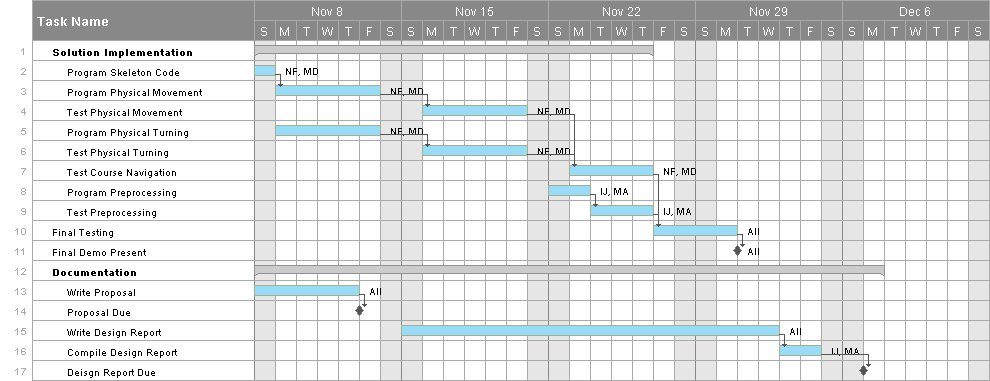
\includegraphics[angle=90,origin=c,width=0.5\textwidth]{images/GanttChart.PNG}
\hspace*{\fill}
\end{document}